\documentclass[
  ngerman,
  color=8c,
  submission,
  boxarc,
  fleqn,
]{rubos-tuda-template}

\usepackage{drawstack}
\usepackage{pgfplots}
\usepackage{tabularray}

\groupnumber{3}
\addSubmittor{Bora Büyükbas}{}
\addSubmittor{Philip Seitz}{}
\addSubmittor{Fares Elkholy}{}
\groupLeader{<Gruppenleitername>}
\semester{SoSe 2024}
%\version{1.0}
\fachbereich{Informatik}
% \dozent{<Prof>}
\date{\today}
\termStyle{left-right-manual}
\termLeft{%
    printAuthor,%
    printSubmittors,%
}
\termRight{%
    printSheetNumber,%
    %printVersion,%
    printGroupNumber,%
    %printGroupLeader,%
    printSemester,%
}

\begin{document}

\title[Parallele Programmierung]{Performance Analysis für Aufgabe 2n\\ Parallele Programmierung}
\maketitle{}

Für die Performance Analyse unserer Implementierung der naiven CUDA-Simulation soll mit der CPU-parallelen
Barnes-Hut Implementierung ein Performance-Vergleich durchgeführt werden. Die Zusammenstellung der Benchmark-
Ergebnisse, bei der die Laufzeit jeweils für verschiedene Körperanzahlen durchgeführt wurde, ist folgender
Grafik zu entnehmen.

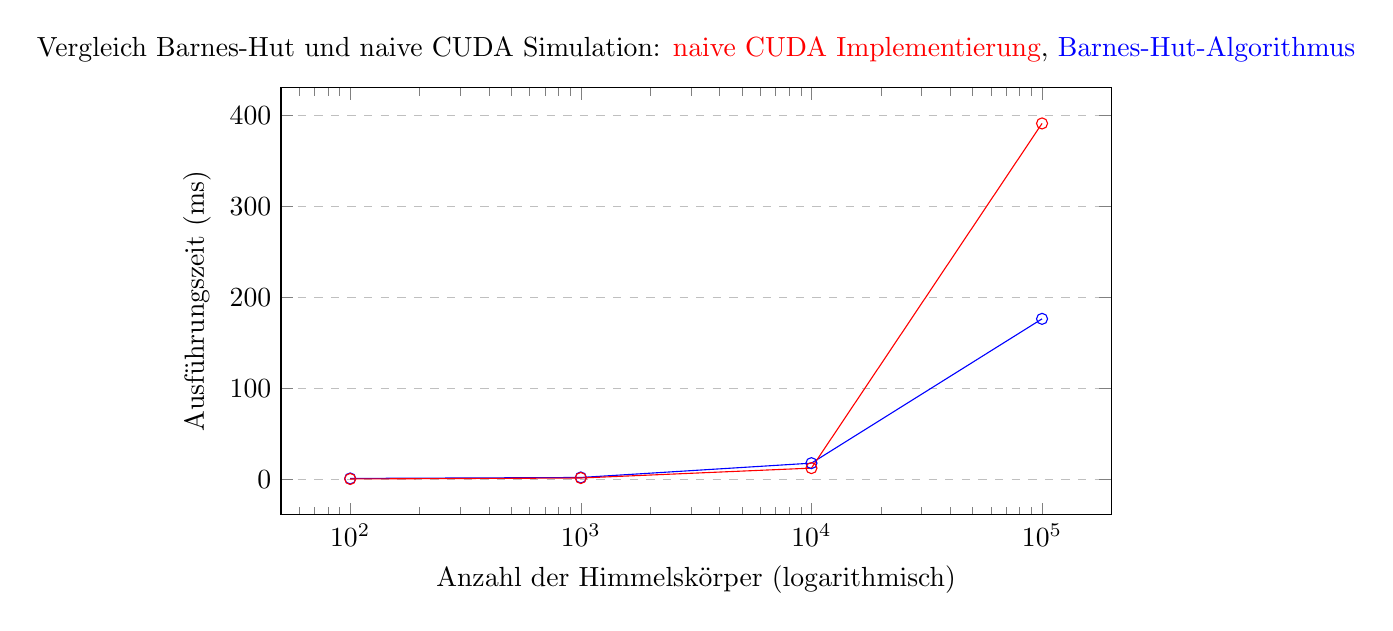
\begin{tikzpicture}
  \begin{axis}[
      xmode=log,
      width=\textwidth,
      height=7cm,
      title={Vergleich Barnes-Hut und naive CUDA Simulation: \textcolor{red}{naive CUDA Implementierung}, \textcolor{blue}{Barnes-Hut-Algorithmus}},
      xlabel={Anzahl der Himmelskörper (logarithmisch)},
      ylabel={Ausführungszeit (ms)},
      % xmin=0, xmax=100,
      % restrict y to domain=0:1000,
      % xtick={0,1,2,3,4,5,6,7,8,9},
      % ytick={0,20,40,60,80,100,120},
      % ymin=-3, ymax=20,
      % ytick={0, 5, 10, 15, 20},
      % restrict y to domain=5:18,
      % ymin=5, ymax=18,
      scaled ticks=false,
      % tick label style={/pgf/number format/fixed},
      legend pos=north west,
      ymajorgrids=true,
      grid style=dashed,
    ]

    \addplot[
      color=blue,
      mark=o,
    ]
    coordinates {
        (100, 0.973)
        (1000, 2.043)
        (10000, 17.777)
        (100000, 176.3)
      };

    \addplot[
      color=red,
      mark=o,
    ]
    coordinates {
        (100, 0.407)
        (1000, 1.460)
        (10000, 12.333)
        (100000, 391)
      };

  \end{axis}
\end{tikzpicture}

Es lässt sich festhalten, dass die CPU parellele Implementierung bei höherer Körperanzahl (ab 100000 Körpern) deutlich geringere
Laufzeit hat. Bei geringerer Körperanzahl schneidet die CUDA Implementierung jedoch besser ab. Das lässt sich damit begründen, dass
die Barnes-Hut Simulation Overhead bezüglich Erstellung des Quadtrees mit sich bringt. Für geringe Anzahlen an Körpern ist diese
natürlich auffällig.

Während der Entwicklung der CUDA Simulation wurde die Feststellung gemacht, dass die Berechnung der Kräfte den größten Laufzeitanteil der Simulation ausmacht.

Für eine hohe Anzahl an Körpern ist somit der Laufzeit-Unterschied der beiden Simulationen auf die Algorithmen zurückzuführen. Während bei
Barnes-Hut effiezient die relevanten Körper für die Berechnung der Kräfte ausgewählt werden, berechnet die CUDA-Simulation Kräfte für alle
Körper (in unserer Implementierung mit Tiling, um effizienteres Speicherverhalten zu erzielen), was trotz Parallelisierung nicht mit dem
Barnes-Hut Algorithmus konkurieren kann.


\end{document}
